\documentclass[]{article}

\usepackage{tikz}
\usetikzlibrary{
    arrows.meta,
    graphs,
    positioning
}
\usepackage{amsmath, amssymb} % for $\therefore e_{l} * e_{r} \implies e_{r}$

% epigraph for quote at start of section
\usepackage{epigraph}
\setlength\epigraphwidth{8cm}
\setlength\epigraphrule{0pt}
\renewcommand{\epigraphsize}{\small\itshape}

% for hyperlinks and URL links
\usepackage{hyperref}

\title{\LaTeX{} Experiments\\ Part III: PGF/TikZ}

\author{AeAeA}

\begin{document}

\maketitle

%==============================================================================
\section{TikZ ist {\itshape kein} Zeichenprogramm}

\epigraph
{Für meinen Vater, damit er noch viele schöne TEX-Graphiken erschaffen kann.}
{--- \textup{Till Tantau}}

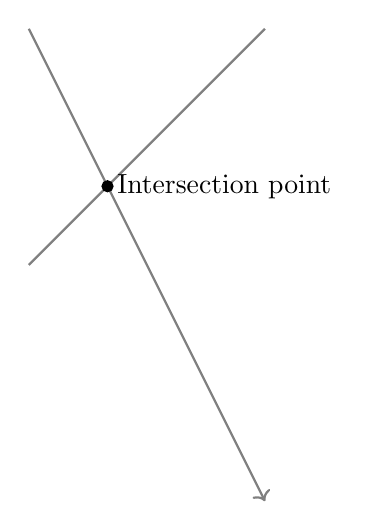
\begin{tikzpicture}
    \draw[gray, thick, ->] (-1,2) -- (2,-4);
    \draw[gray, thick] (-1,-1) -- (2,2);
    \filldraw[black] (0,0) circle (2pt) node[anchor=west] {Intersection point};
\end{tikzpicture}

\begin{itemize}
    \item \url{https://en.wikipedia.org/wiki/PGF/TikZ}
    \item \url{https://www.ctan.org/pkg/pgf}
    \item \url{https://github.com/pgf-tikz/pgf}
    \item \href{http://cremeronline.com/LaTeX/minimaltikz.pdf}
               {Minimal introduction to TikZ (unofficial)}
    \item  It comes with very good documentation; the version 3.1.5b of the 
           \href{http://mirrors.ctan.org/graphics/pgf/base/doc/pgfmanual.pdf}
                {PGF Manual} has over 1,300 pages (!) \ldots
    \item \ldots and an extensive collection of examples: \\
          \url{http://www.texample.net/tikz/}
    \item \url{https://en.wikibooks.org/wiki/LaTeX/PGF/TikZ}
    \item \url{https://www.overleaf.com/learn/latex/TikZ_package}
\end{itemize}

%--------------------------------------
\subsection{Basic elements: points, lines and paths}

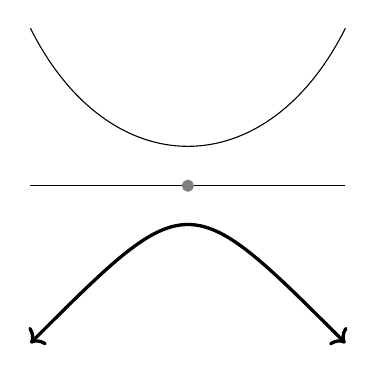
\begin{tikzpicture}
    \draw (-2,0) -- (2,0);
    \filldraw [gray] (0,0) circle (2pt);
    \draw[very thick, <->] (-2,-2) .. controls (0,0) .. (2,-2);
    \draw (-2,2) .. controls (-1,0) and (1,0) .. (2,2); 
\end{tikzpicture}

%--------------------------------------
\subsection{Basic geometric shapes: Circles, ellipses and polygons}

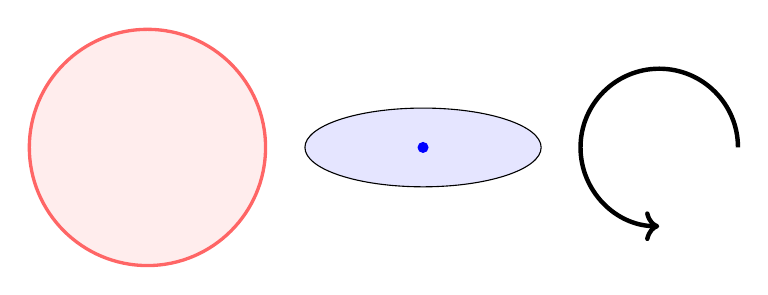
\begin{tikzpicture}
    \filldraw[color=red!60, fill=red!7, very thick] (-1,0) circle (1.5);
    \fill[blue!10] (2.5,0) ellipse (1.5 and 0.5);
    \fill[blue]    (2.5,0) circle (2pt);
    \draw (2.5,0) ellipse [x radius=1.5, y radius=0.5];
    \draw[ultra thick, ->] (6.5,0) arc (0:270:1);
\end{tikzpicture}

\vspace{20pt}

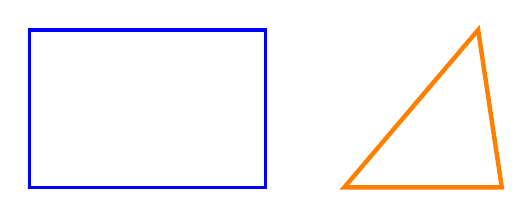
\begin{tikzpicture}
    \draw[blue, very thick] (0,0) rectangle (3,2);
    \draw[orange, ultra thick] (4,0) -- (6,0) -- (5.7,2) -- cycle;
\end{tikzpicture}

The code for the little "turned" ellipse 
\tikz \draw[rotate=30] (0,0) ellipse [x radius=6pt,y radius=3pt]; is \\
\verb+\tikz \draw[rotate=30] (0,0) ellipse [x radius=6pt,y radius=3pt];+

%--------------------------------------
\subsection{Elliptical arc}
%  \usetikzlibrary {arrows.meta}
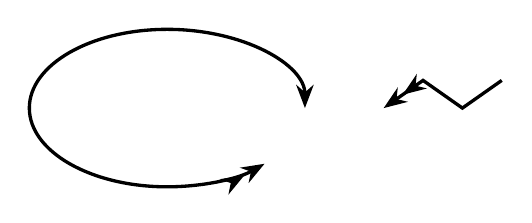
\begin{tikzpicture}[>=Stealth]
    \draw[<->>,very thick] 
        (0,0) arc [start angle=0, end angle=315, x radius=1.75cm, y radius=1cm];
    \draw[<<-,very thick] (1,0) -- (1.5cm,10pt) -- (2cm,0pt) -- (2.5cm,10pt);
\end{tikzpicture}

%--------------------------------------
\subsection{Arrow tips}
%  \usetikzlibrary {arrows.meta}
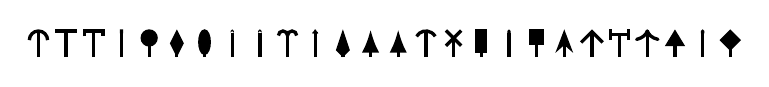
\begin{tikzpicture} [->,very thick]
    \draw[>=Arc Barb]      (0,0) -- (0,10pt);
    \draw[>=Bar]           (10pt,0) -- (10pt,10pt);
    \draw[>=Bracket]       (20pt,0) -- (20pt,10pt);
    \draw[>=Butt Cap]      (30pt,0) -- (30pt,10pt);
    \draw[>=Circle]        (40pt,0) -- (40pt,10pt);
    \draw[>=Diamond]       (50pt,0) -- (50pt,10pt);
    \draw[>=Ellipse]       (60pt,0) -- (60pt,10pt);
    \draw[>=Fast Round]    (70pt,0) -- (70pt,10pt);
    \draw[>=Fast Triangle] (80pt,0) -- (80pt,10pt);
    \draw[>=Hooks]         (90pt,0) -- (90pt,10pt);
    \draw[>=Implies]       (100pt,0) -- (100pt,10pt);
    \draw[>=Kite]          (110pt,0) -- (110pt,10pt);
    \draw[>=LaTeX]         (120pt,0) -- (120pt,10pt);
    \draw[>=Latex]         (130pt,0) -- (130pt,10pt);
    \draw[>=Parenthesis]   (140pt,0) -- (140pt,10pt);
    \draw[>=Rays]          (150pt,0) -- (150pt,10pt);
    \draw[>=Rectangle]     (160pt,0) -- (160pt,10pt);
    \draw[>=Round Cap]     (170pt,0) -- (170pt,10pt);
    \draw[>=Square]        (180pt,0) -- (180pt,10pt);
    \draw[>=Stealth]       (190pt,0) -- (190pt,10pt);
    \draw[>=Straight Barb] (200pt,0) -- (200pt,10pt);
    \draw[>=Tee Barb]      (210pt,0) -- (210pt,10pt);
    \draw[>=To]            (220pt,0) -- (220pt,10pt);
    \draw[>=Triangle]      (230pt,0) -- (230pt,10pt);
    \draw[>=Triangle Cap]  (240pt,0) -- (240pt,10pt);
    \draw[>=Turned Square] (250pt,0) -- (250pt,10pt);
\end{tikzpicture}

\subsubsection{Arrow Tip Kind \texttt{Implies}}
\marginpar{$\therefore\\ e_{l} * e_{r} \implies e_{r}$}
This arrow tip makes only sense in conjunction with the double option:
attach it to a double line to get something 
( \tikz \draw[double equal sign distance, -Implies] (0,0) -- (15pt,0); ) 
that looks like 
\texttt{amsmath} \TeX’s \verb+\implies+ arrow ( $\implies$ ). 
A typical use of this arrow tip is:\\
% \usetikzlibrary {arrows.meta,graphs}
\tikz \graph [
    clockwise=3, math nodes, edges = {double equal sign distance, -Implies}
] { 
    "\alpha", "\beta", "\gamma";
    "\alpha" -> "\beta" -> "\gamma" -> "\alpha"
};



%--------------------------------------
\subsection{Diagrams with nodes}

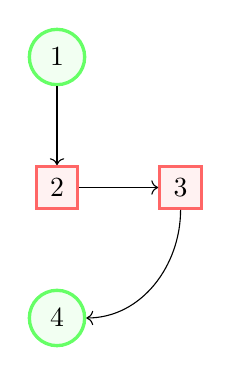
\begin{tikzpicture}[
    roundnode/.style   = {circle, draw=green!60, fill=green!5, very thick, 
                          minimum size=20pt},
    squarednode/.style = {rectangle, draw=red!60, fill=red!5, very thick, 
                          minimum size=15pt},
]
    %Nodes
    \node[squarednode]      (maintopic)                              {2};
    \node[roundnode]        (uppercircle)       [above=of maintopic] {1};
    \node[squarednode]      (rightsquare)       [right=of maintopic] {3};
    \node[roundnode]        (lowercircle)       [below=of maintopic] {4};
     
    %Lines
    \draw[->] (uppercircle.south) -- (maintopic.north);
    \draw[->] (maintopic.east) -- (rightsquare.west);
    \draw[->] (rightsquare.south) .. 
              controls +(down:20pt) and +(right:20pt) 
              .. (lowercircle.east);
\end{tikzpicture}

\subsubsection{Extracting Insights From Data diagram}
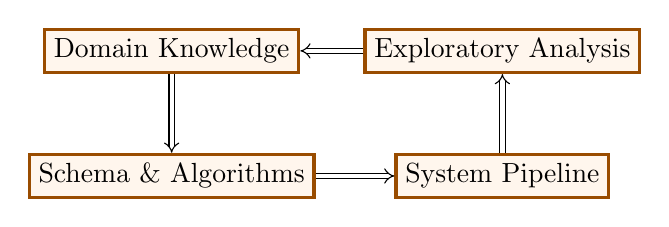
\begin{tikzpicture}[
    squarednode/.style = {rectangle, draw=orange!60!black, fill=orange!7, 
                          very thick, 
                          minimum size=15pt},
    impliesarrow/.style = {double equal sign distance, -Implies}
]
  
    \node[squarednode] (DK) {Domain Knowledge};
    \node[squarednode] (SA) [below=of DK] {Schema \& Algorithms};
    \node[squarednode] (SP) [right=of SA] {System Pipeline};
    \node[squarednode] (EA) [above=of SP] {Exploratory Analysis};

    \draw[impliesarrow] (DK.south) -- (SA.north);
    \draw[impliesarrow] (SA.east) -- (SP.west);
    \draw[impliesarrow] (SP.north) -- (EA.south);
    \draw[impliesarrow] (EA.west) -- (DK.east);
    % \draw[impliesarrow] (DA.north) .. controls +(up:30pt) and +(right:40pt) .. (DK.east);

\end{tikzpicture}


%--------------------------------------
\subsection{Path}

\tikz \draw[thick,rounded corners=8pt]
    (0,0) -- (0,2) -- (1,3.25) -- (2,2) -- (2,0) -- (0,2) -- (2,2) -- (0,0) -- (2,0);

%--------------------------------------
\subsection{Curved path}

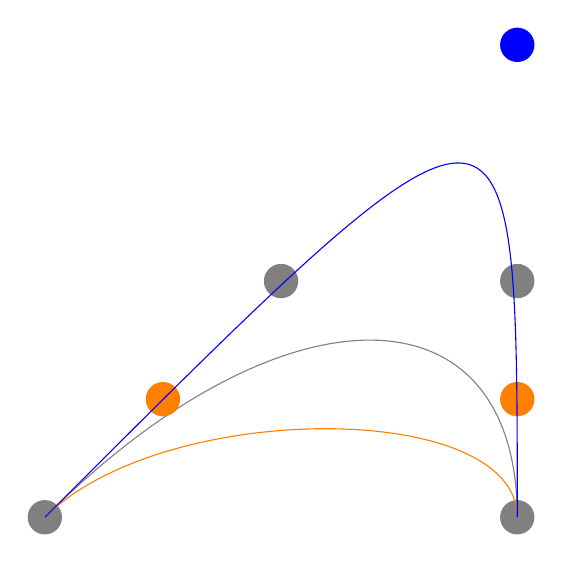
\begin{tikzpicture}[scale=3]
    \filldraw[gray] (0,0) circle [radius=2pt]
                    (1,1) circle [radius=2pt] 
                    (2,1) circle [radius=2pt] 
                    (2,0) circle [radius=2pt];
    \draw[gray] (0,0) .. controls (1,1) and (2,1) .. (2,0);

    \filldraw[orange] (0.5,0.5) circle [radius=2pt]
                      (2,0.5) circle [radius=2pt];                
    \draw[orange] (0,0) .. controls (0.5,0.5) and (2,0.5) .. (2,0);

    \filldraw[blue] (2,2) circle [radius=2pt];
    \draw[blue] (0,0) .. controls (2,2) .. (2,0);
\end{tikzpicture}

%--------------------------------------
\subsection{Grid}
The code \verb+\tikz \draw[step=2pt] (0,0) grid (10pt,10pt);+ produces
\tikz \draw[step=2pt] (0,0) grid (10pt,10pt);.

Here is a bigger grid:\\
\tikz{ 
    \fill[orange] (0,0) circle (2pt);
    \fill[red] (50pt,50pt) circle (2pt);
    \fill[blue] (100pt,100pt) circle (2pt);

    \draw[step=5pt,gray,very thin] (1pt,1pt) grid (99pt,99pt);

    \draw (50pt,0) -- (50pt,100pt); % vertical
    \draw (0,50pt) -- (100pt,50pt); % horizontal
}

%--------------------------------------
\subsection{Circle and curved path}
0.555 is the magic number.\\
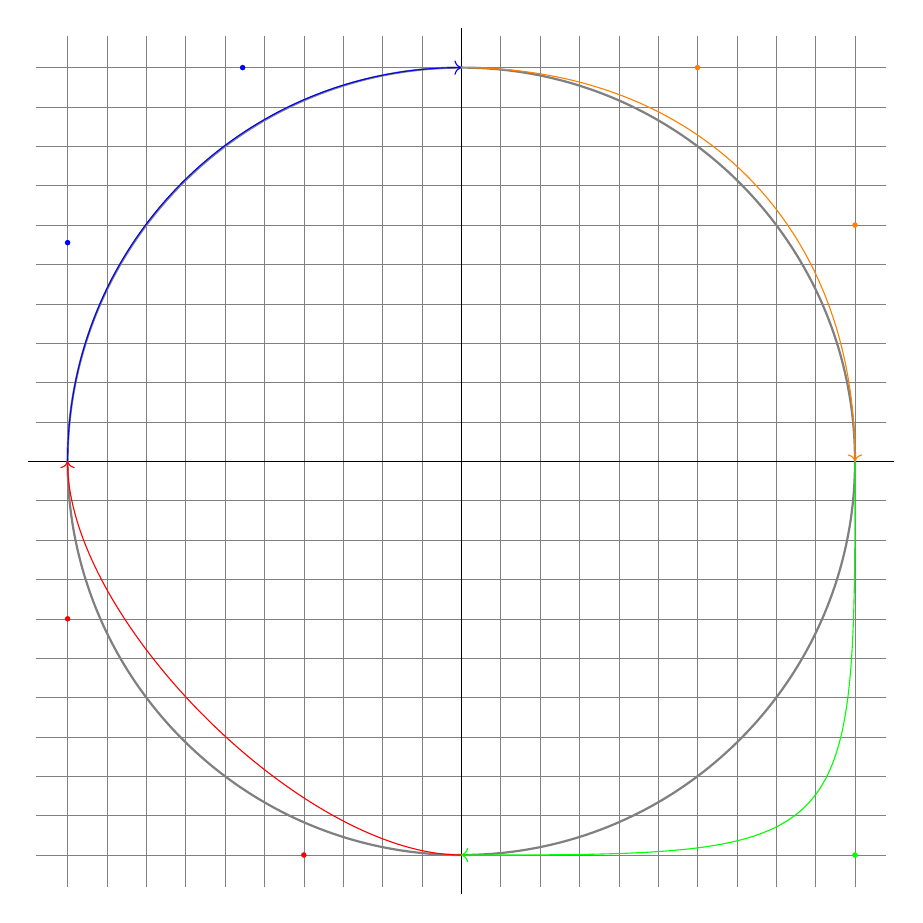
\begin{tikzpicture}
    \draw[step=.5cm,gray,very thin] (-5.4,-5.4) grid (5.4,5.4); 

    \draw (-5.5,0) -- (5.5,0);
    \draw (0,-5.5) -- (0,5.5);

    \draw[gray,thick] (0,0) circle [radius=5cm];

    \fill[blue] (-5,2.777) circle (1pt) (-2.777,5) circle (1pt);
    \draw[blue,->] (-5,0) .. controls (-5,2.777) and (-2.777,5) .. (0,5);

    \fill[orange] (3,5) circle (1pt) (5,3) circle (1pt);
    \draw[orange,->] (0,5) .. controls (3,5) and (5,3) .. (5,0);

    \fill[green] (5,-5) circle (1pt);
    \draw[green,->] (5,0) .. controls (5,-5) .. (0,-5);

    \fill[red] (-2,-5) circle (1pt) (-5,-2) circle (1pt);
    \draw[red,->] (0,-5) .. controls (-2,-5) and (-5,-2) .. (-5,0);
\end{tikzpicture}

%--------------------------------------
\subsection{Style}
\tikzset{help lines/.style=very thin}
\begin{tikzpicture}[
    Karl's grid/.style ={help lines,color=#1!50},
    Karl's grid/.default=blue
]

    \draw[Karl's grid]     (0,0) grid (1.5,2);
    \draw[Karl's grid=red] (2,0) grid (3.5,2);
\end{tikzpicture}

%--------------------------------------
\subsection{Clipping a path}
Original drawing on the left, clipped drawing on the right:\\
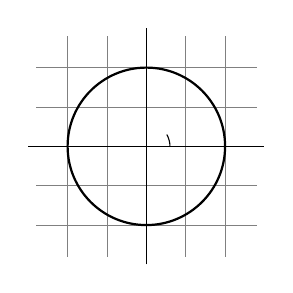
\begin{tikzpicture}
    \draw[step=.5cm,gray,very thin] (-1.4,-1.4) grid (1.4,1.4); 
    \draw (-1.5,0) -- (1.5,0);
    \draw (0,-1.5) -- (0,1.5);
    \draw[thick] (0,0) circle [radius=1cm];
    \draw (3mm,0mm) arc [start angle=0, end angle=30, radius=3mm];
\end{tikzpicture}
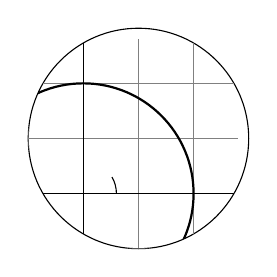
\begin{tikzpicture}[scale=1.4]
    \path[draw,clip] (0.5,0.5) circle (1cm);
    \draw[step=.5cm,gray,very thin] (-1.4,-1.4) grid (1.4,1.4); 
    \draw (-1.5,0) -- (1.5,0);
    \draw (0,-1.5) -- (0,1.5);
    \draw[thick] (0,0) circle [radius=1cm];
    \draw (3mm,0mm) arc [start angle=0, end angle=30, radius=3mm];
\end{tikzpicture}

%--------------------------------------
\subsection{Parabola and Sine}
Two parabolas 
\tikz \draw[x=2ex,y=2ex] (-1,0) rectangle (1,1) (-1,1) parabola (0,0) parabola (1,1);
and a parabola with placed bend 
\tikz \draw[x=2ex,y=2ex] (-1,0) rectangle (1,1) (-1,1) parabola bend (0,0) (1,1);

A parabola with the bend:
\tikz \draw[x=1pt,y=1pt] (0,0) parabola bend (4,16) (6,12);

A sine \tikz \draw[x=1ex,y=1ex] (0,0) sin (1.57,1); curve, 
and a longer span of sine and cosine: 
\tikz \draw[x=1.57ex,y=1ex] (0,0) sin (1,1) cos (2,0) sin (3,-1) cos (4,0) 
                            (0,1) cos (1,0) sin (2,-1) cos (3,0) sin (4,1);

%--------------------------------------
\subsection{Closing the path}
The \texttt{--cycle} causes the current path to be closed (actually the current part of 
the current path) by smoothly joining the first and last point. To appreciate 
the difference, consider the following example:\\
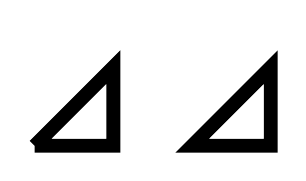
\begin{tikzpicture}[line width=5pt]
    \draw (0,0) -- (1,0) -- (1,1) -- (0,0);
    \draw (2,0) -- (3,0) -- (3,1) -- cycle; 
    \useasboundingbox (0,1.5); % make bounding box higher
\end{tikzpicture}

%--------------------------------------
\subsection{Shading}
The default shading is a smooth transition from gray at the top 
to white at the bottom:\\
\tikz \shade (0,0) rectangle (2,1)  (3,0.5) circle (.5cm);

To specify different colors, you can use options:\\ 
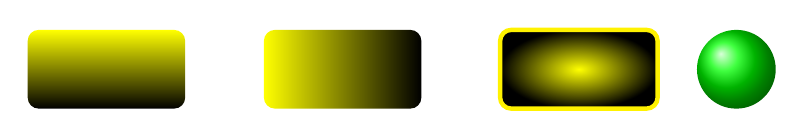
\begin{tikzpicture}[rounded corners,ultra thick]
    \shade[top color=yellow,bottom color=black] (0,0) rectangle +(2,1);
    \shade[left color=yellow,right color=black] (3,0) rectangle +(2,1);
    \shadedraw[inner color=yellow,outer color=black,draw=yellow] (6,0) rectangle +(2,1); \shade[ball color=green] (9,.5) circle (.5cm);
\end{tikzpicture}

%--------------------------------------
\subsection{Scoping}
\begin{tikzpicture}[ultra thick]
    \draw (0,0) -- (0,1);
    \begin{scope}[thin]
        \draw (1,0) -- (1,1);
        \draw (2,0) -- (2,1);
    \end{scope}
    \draw (3,0) -- (3,1);
\end{tikzpicture}

%--------------------------------------
\subsection{Specifying Coordinates}
To appreciate the difference between + and ++ consider the following example:\\
\verb|-- ++(1cm,0cm)  -- ++(0cm,1cm)  -- ++(-1cm,0cm) -- cycle|\\
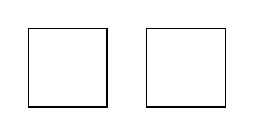
\begin{tikzpicture}
    \def\rectanglepath{-- ++(1cm,0cm)  -- ++(0cm,1cm)  -- ++(-1cm,0cm) -- cycle}
    \draw (0,0) \rectanglepath;
    \draw (1.5,0) \rectanglepath;
\end{tikzpicture}

By comparison, when using a single +, the coordinates are different:\\
\verb|-- +(1cm,0cm)  -- +(1cm,1cm)  -- +(0cm,1cm) -- cycle|\\
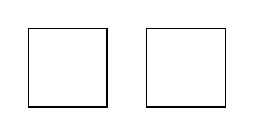
\begin{tikzpicture}
    \def\rectanglepath{-- +(1cm,0cm)  -- +(1cm,1cm)  -- +(0cm,1cm) -- cycle}
    \draw (0,0) \rectanglepath;
    \draw (1.5,0) \rectanglepath;
\end{tikzpicture}

%--------------------------------------
\subsection{Transformations}
\tikz \draw (0,0) -- (0,0.5) [xshift=20pt] (0,0) -- (0,0.5);

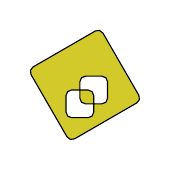
\begin{tikzpicture}[even odd rule,rounded corners=2pt,x=10pt,y=10pt] 
    \filldraw[fill=yellow!80!black] (0,0) rectangle (1,1) 
            [xshift=5pt,yshift=5pt] (0,0) rectangle (1,1)
                      [rotate=30] (-1,-1) rectangle (2,2);
\end{tikzpicture}

Another way to display all options for arrow tips:\\
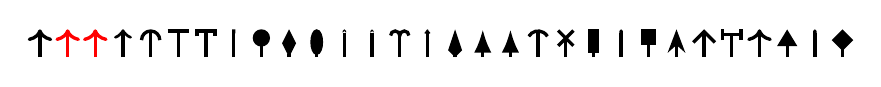
\begin{tikzpicture}
    %  \usetikzlibrary {arrows.meta}
    \def\arrowup{[->,very thick] (0,0) -- (0,10pt)}

    \draw                                   [xshift=-40pt] \arrowup;
    \draw[>=To,red]                         [xshift=-30pt] \arrowup;
    \draw[>=Computer Modern Rightarrow,red] [xshift=-20pt] \arrowup;
    \draw[>=Classical TikZ Rightarrow]      [xshift=-10pt] \arrowup;

    \draw[>=Arc Barb]                    \arrowup;
    \draw[>=Bar]           [xshift=10pt] \arrowup;
    \draw[>=Bracket]       [xshift=20pt] \arrowup;
    \draw[>=Butt Cap]      [xshift=30pt] \arrowup;
    \draw[>=Circle]        [xshift=40pt] \arrowup;
    \draw[>=Diamond]       [xshift=50pt] \arrowup;
    \draw[>=Ellipse]       [xshift=60pt] \arrowup;
    \draw[>=Fast Round]    [xshift=70pt] \arrowup;
    \draw[>=Fast Triangle] [xshift=80pt] \arrowup;
    \draw[>=Hooks]         [xshift=90pt] \arrowup;
    \draw[>=Implies]       [xshift=100pt] \arrowup;
    \draw[>=Kite]          [xshift=110pt] \arrowup;
    \draw[>=LaTeX]         [xshift=120pt] \arrowup;
    \draw[>=Latex]         [xshift=130pt] \arrowup;
    \draw[>=Parenthesis]   [xshift=140pt] \arrowup;
    \draw[>=Rays]          [xshift=150pt] \arrowup;
    \draw[>=Rectangle]     [xshift=160pt] \arrowup;
    \draw[>=Round Cap]     [xshift=170pt] \arrowup;
    \draw[>=Square]        [xshift=180pt] \arrowup;
    \draw[>=Stealth]       [xshift=190pt] \arrowup;
    \draw[>=Straight Barb] [xshift=200pt] \arrowup;
    \draw[>=Tee Barb]      [xshift=210pt] \arrowup;
    \draw[>=To]            [xshift=220pt] \arrowup;
    \draw[>=Triangle]      [xshift=230pt] \arrowup;
    \draw[>=Triangle Cap]  [xshift=240pt] \arrowup;
    \draw[>=Turned Square] [xshift=250pt] \arrowup;
\end{tikzpicture}

\end{document}